\chapter{Implementation and Testing} \label{ch:implementation}
This chapter explains the development approach used followed by how each element of the design was implemented.


\section{Development approach} 
\label{sec:developmentapproach}
The software was developed through evolutionary prototyping. Since the initial requirements were not complete, this approach gave flexibility on what is to be implemented. Unlike throwaway prototyping where code is thrown away, this method begins with the requirements that are understood and seeks to incrementally implement additional features proposed by the user (citation). Though the usual definition is to modify the software based on feedback from the user, I have taken the place of the user and have incrementally designed and then implemented what is most likely suitable for the users\textsc{\char13} analysis of the data. Therefore, the interaction and interface designs of the application were created incrementally and the design as a whole was added in the Design chapter.\par

The following list outlines the iterations of the prototype including the requirements that were implemented:
\begin{itemize}
	\item Implementation of groups in the population and graph visualizations of certain questions, group\_detail.html and group\_new.html using the residential survey data only (Functional Requirements 1, 2a, 2bi, 2bii, 2biv, 2e)
	\item Addition of survey code translations to the visualizations implemented in the iteration 1.
	\item Implementation of resources\_list and resource\_datafields.html
	\item Implementation of the map in group\_detail.html (Functional Requirements 2iii, 2c)
	\item Implementation of the group\_compare.html (Functional Requirement 2d)
	\item Implementation of clustering and cluster\_detail.html (Functional Requirement 3a)
	\item Implementation of the interface cluster\_stats (Functional Requirement 3b, 3c)
	\item Implementation of the interface cluster\_compare.html (Funcitonal Requirement 3c)
\end{itemize}

The implementation stated with the initial requirements and each succeeding increment involved design, implementation and testing. The functional requirements were relatively done in order it was listed since each requirement usually depended on the previous requirement. The function and interface of each page was done together so that each prototype is functional. The prototype could then be tested and features for the next prototype could be suggested, which follows the spirit of evolutionary prototyping. \par 

Development involved developing sections of the prototype that was independent of the system for some iterations. This was to familiarize myself to the different languages and libraries used in this application, which lead to the creation of an independently functioning section of the prototype. This was then integrated into the system to avoid confusion with other parts of the code. Independently developing it ensured that it was functional before it was integrated. This also reduced the risk of it not working.  An example is the integration of a Google Map and the Google Charts used in group\_detail.html. The clicking of a chart and display on the map was implemented in a separate HTML page and ensured that it worked. This was then integrated into the actual page, group\_detail.html. The user friendliness was also improved through this method, as testing the interfaces in reality makes missing user friendly elements more obvious than could be seen in the design of the interfaces.

\section{Third party libraries}
The third party libraries are listed below:
\begin{itemize}
    \item Django: a Python web framework used to create web applications
    \item Bootstrap: a CSS library used to make webpages more aesthetically pleasing
    \item Pandas (citation): a Python library used for data analysis and data structures
    \item Google Charts: a JavaScript API which creates different types of charts
    \item Google Maps: a JavaScript API which creates a map
    \item Graphos (citation): a Django app which turns data in the form of Python\textquotesingle s list data structure into Google Charts JavaScript code
•	K-modes: a Python library which applies a clustering algorithm most suited for categorical data on a set of data
\end{itemize}
Since it is a web application, a combination of programming languages were used, Python for the back-end with Django, HTML and CSS for the layout aesthetics of the web page and JavaScript to make the pages interactive.


\section{Page implementations}
The subsections below describe how each part of the software was implemented and some screenshots of the actual implementation.

\subsection{Visualization of data into charts}
Pandas Dataframe was used to store the Residential Survey data. The survey data as a CSV was loaded into a Dataframe and the latter was used to query the data around the system. A single instance of the Dataframe was kept to refrain from repetitively opening and reading the same file through the singleton design pattern.\par

Graphos was used to create the Google Charts. The required data of a chart was queried and formatted to Graphos\textsc{\char13} specficiations and a Graphos object was created. Since Django is a web framework, it has a template feature where Python objects, such as a Graphos graph object, could be turned into content for an HTML file.\par

Depending on the type of question, the charts on figure \ref{fig:4charts} was created.

\begin{figure}[h]
\centering
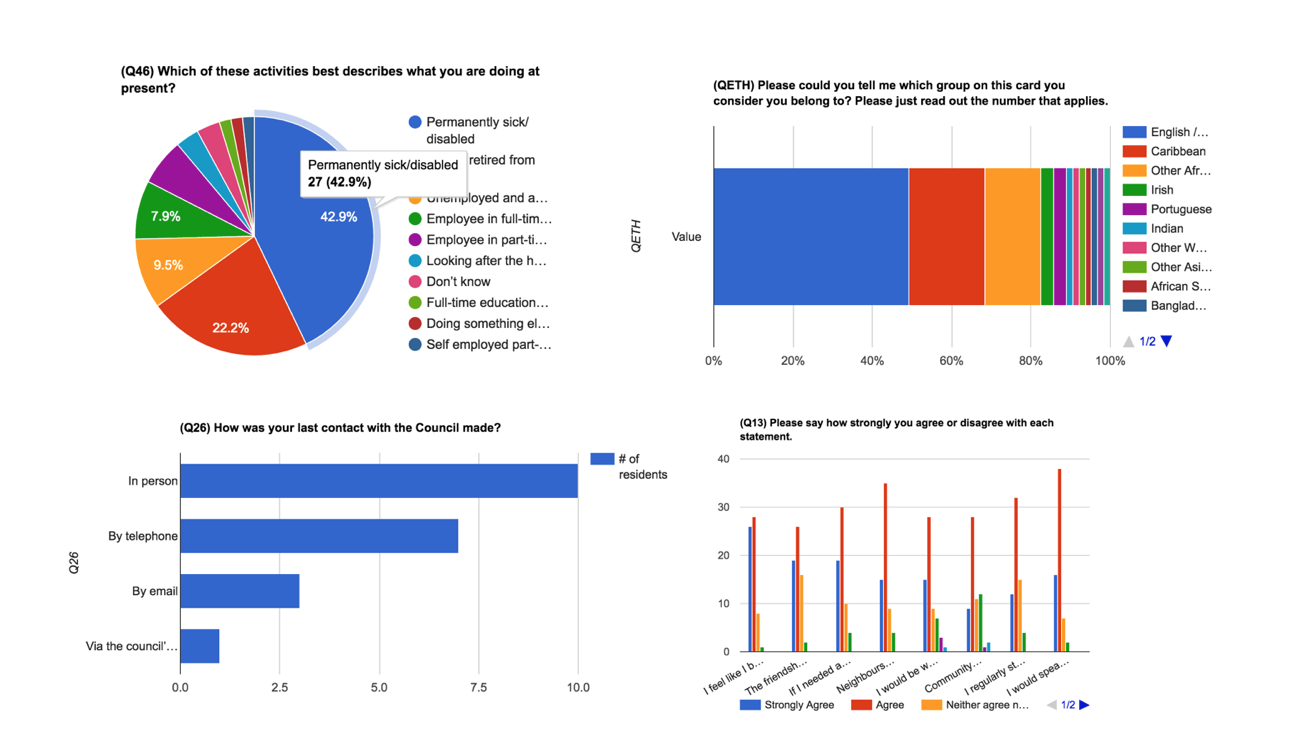
\includegraphics[scale=0.7]{4charts}
\caption{Implementation of the charts}
\label{fig:4charts}
\end{figure}

As a default feature of Google Charts, hovering over a piece of data will display the value of data (see top left of figure \ref{fig:4charts}).

\subsection{Integration of survey code}
Following the design for the preprocessing of data (see figure \ref{fig:figure1}), the English Code translation text file was created. To speed up the creation of this file, the tables were copied into the text file and a small program was created to format the tables, whose elements are spaced by `\textbackslash r', and replaced with a `\textbackslash n' to format the spaces correctly. The rest of the file was typed manually.\par

Readtext.py is the Python module which reads and creates each question into Question objects. Readcsv.py consolidates English and code data into a Python list. This is inputted into a Graphos class which produces the Google Charts JavaScript code. 

\begin{figure}[h]
\centering
\includegraphics[scale=0.5]{figure1.png}
\caption{Implementation of the charts}
\label{fig:figure1}
\end{figure}

Figure \ref{fig:figure1} shows the data flow from raw data to the creation of Graphos charts. This is a simplified view which omits other Django modules.

\subsection{Visualization of wards on a map and ward breakdown chart}

The map was adapted from a tutorial in the Google Maps website which implemented the display of colored areas depending on the value of that area. In this case, the areas were changed to Lambeth\textquotesingle s wards.\par

The interactivity between the Google Map and Google Chart in the group\_detail page was developed as described in Development approach (see section \ref{sec:developmentapproach}). \par

Additional features to the Graphos code was added. A listener to see if the chart was clicked was added to Graphos\textsc{\char13} code. When a chart is clicked, the function which redraws the chart, map and changes the text is invoked. \par

\begin{figure}[h]
\centering
\includegraphics[scale=0.5]{figure2.png}
\caption{Implementation of the charts}
\label{fig:figure1}
\end{figure}

This interactivity required the map\textquotesingle s contents to be changed (i.e. change the colors of the wards depending on the question selected). A JSON containing a list, which is required in the creation of Google Maps, is populated with the selected data from a chart (see figure \ref{fig:figure2}). This JSON is requested by clicking a chart on the right hand side of the page, which invokes the redrawing of the map. The figure below explains the data flow.


\begin{figure}[h]
\centering
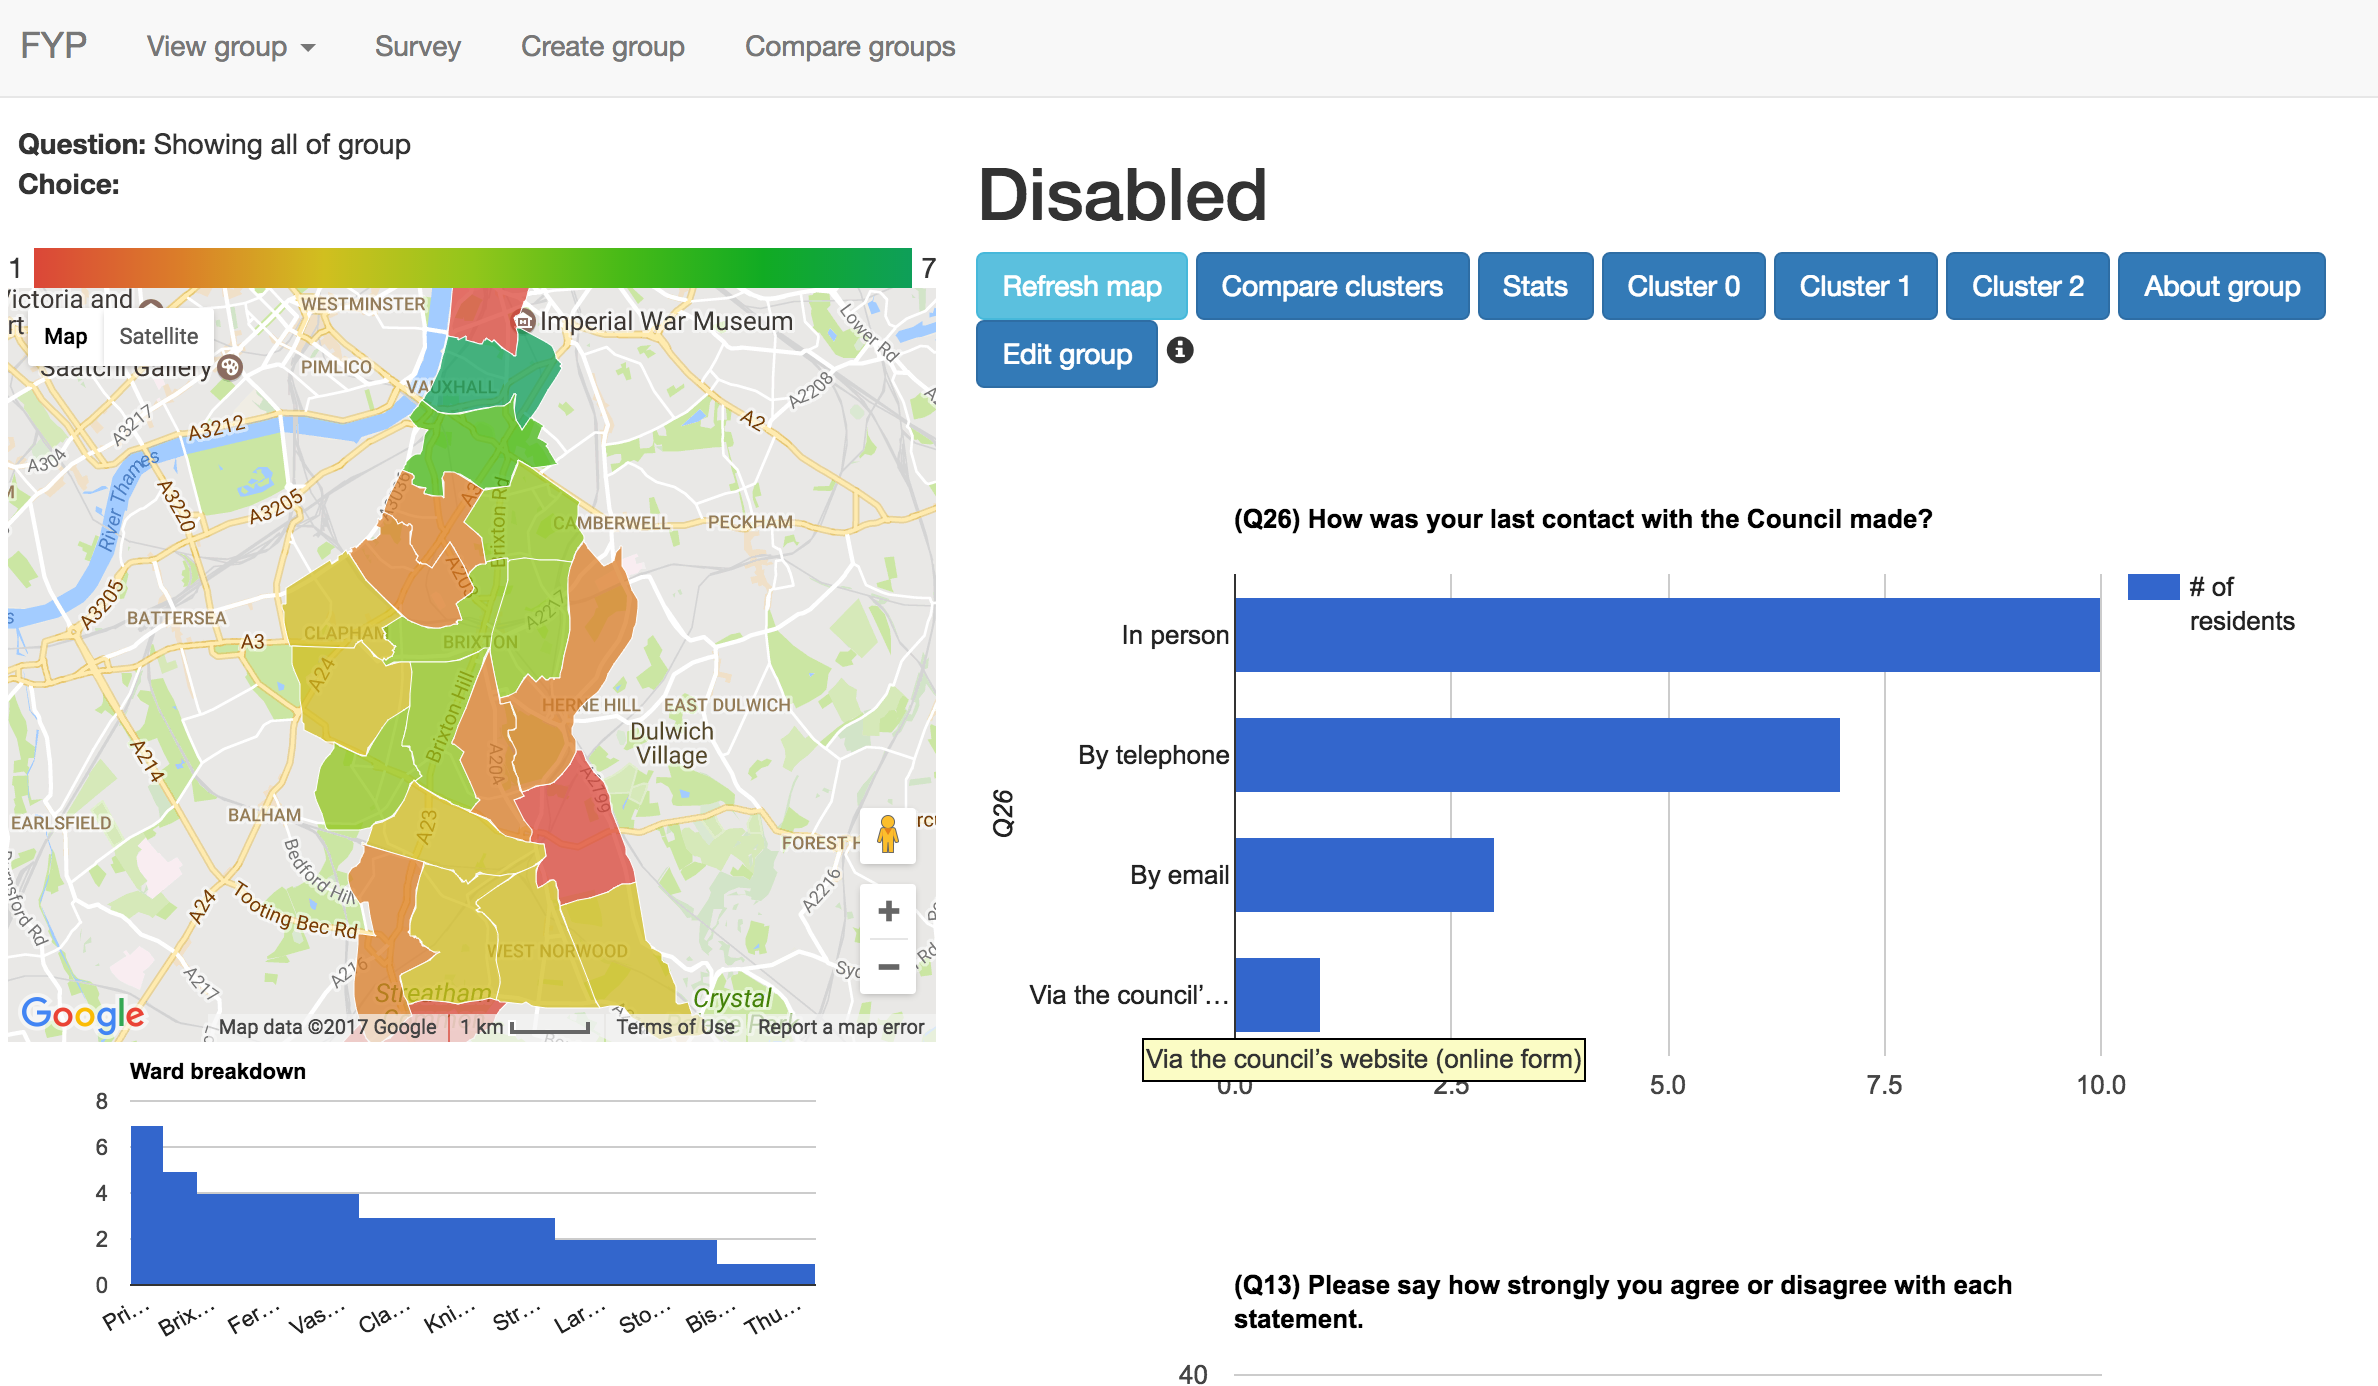
\includegraphics[scale=0.3]{figure3.png}
\caption{Screenshot of the group\_detail page}
\label{fig:figure1}
\end{figure}

Hovering over the map\textquotesingle s wards will display a box containing the ward\textquotesingle s name and value on the bottom left hand side of the map (see figure \ref{fig:hover}).

\begin{figure}[h]
\centering
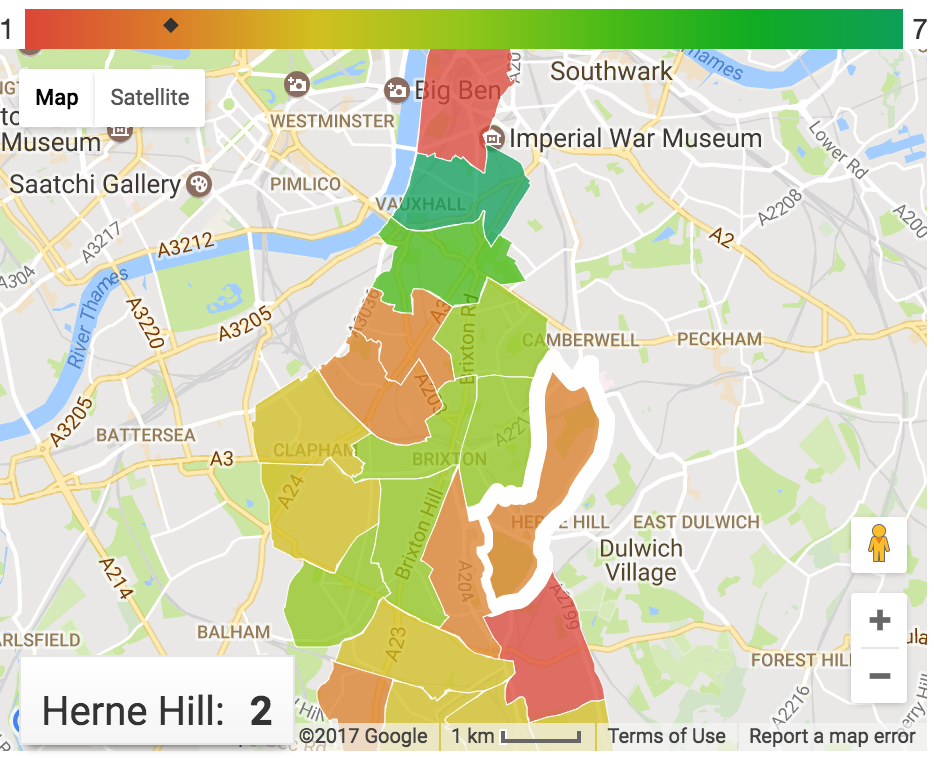
\includegraphics[scale=0.3]{hover}
\caption{Screenshot of hovering over a ward on the Google Map}
\label{fig:hover}
\end{figure}

\subsection{Visualization the Comparison of Clusters}
A group\textquotesingle s data, the whole survey data and clusters\textsc{\char13} data were visualized together for each question in a similar method to the visualization of a single group. To differentiate between each of the clusters\textsc{\char13} data for each question, the cluster id was included into the chart array. This was kept hidden when the array is displayed on the chart, but it is used to know which cluster is clicked when the user wants to display a particular variable on the map.   

\begin{figure}[h]
\centering
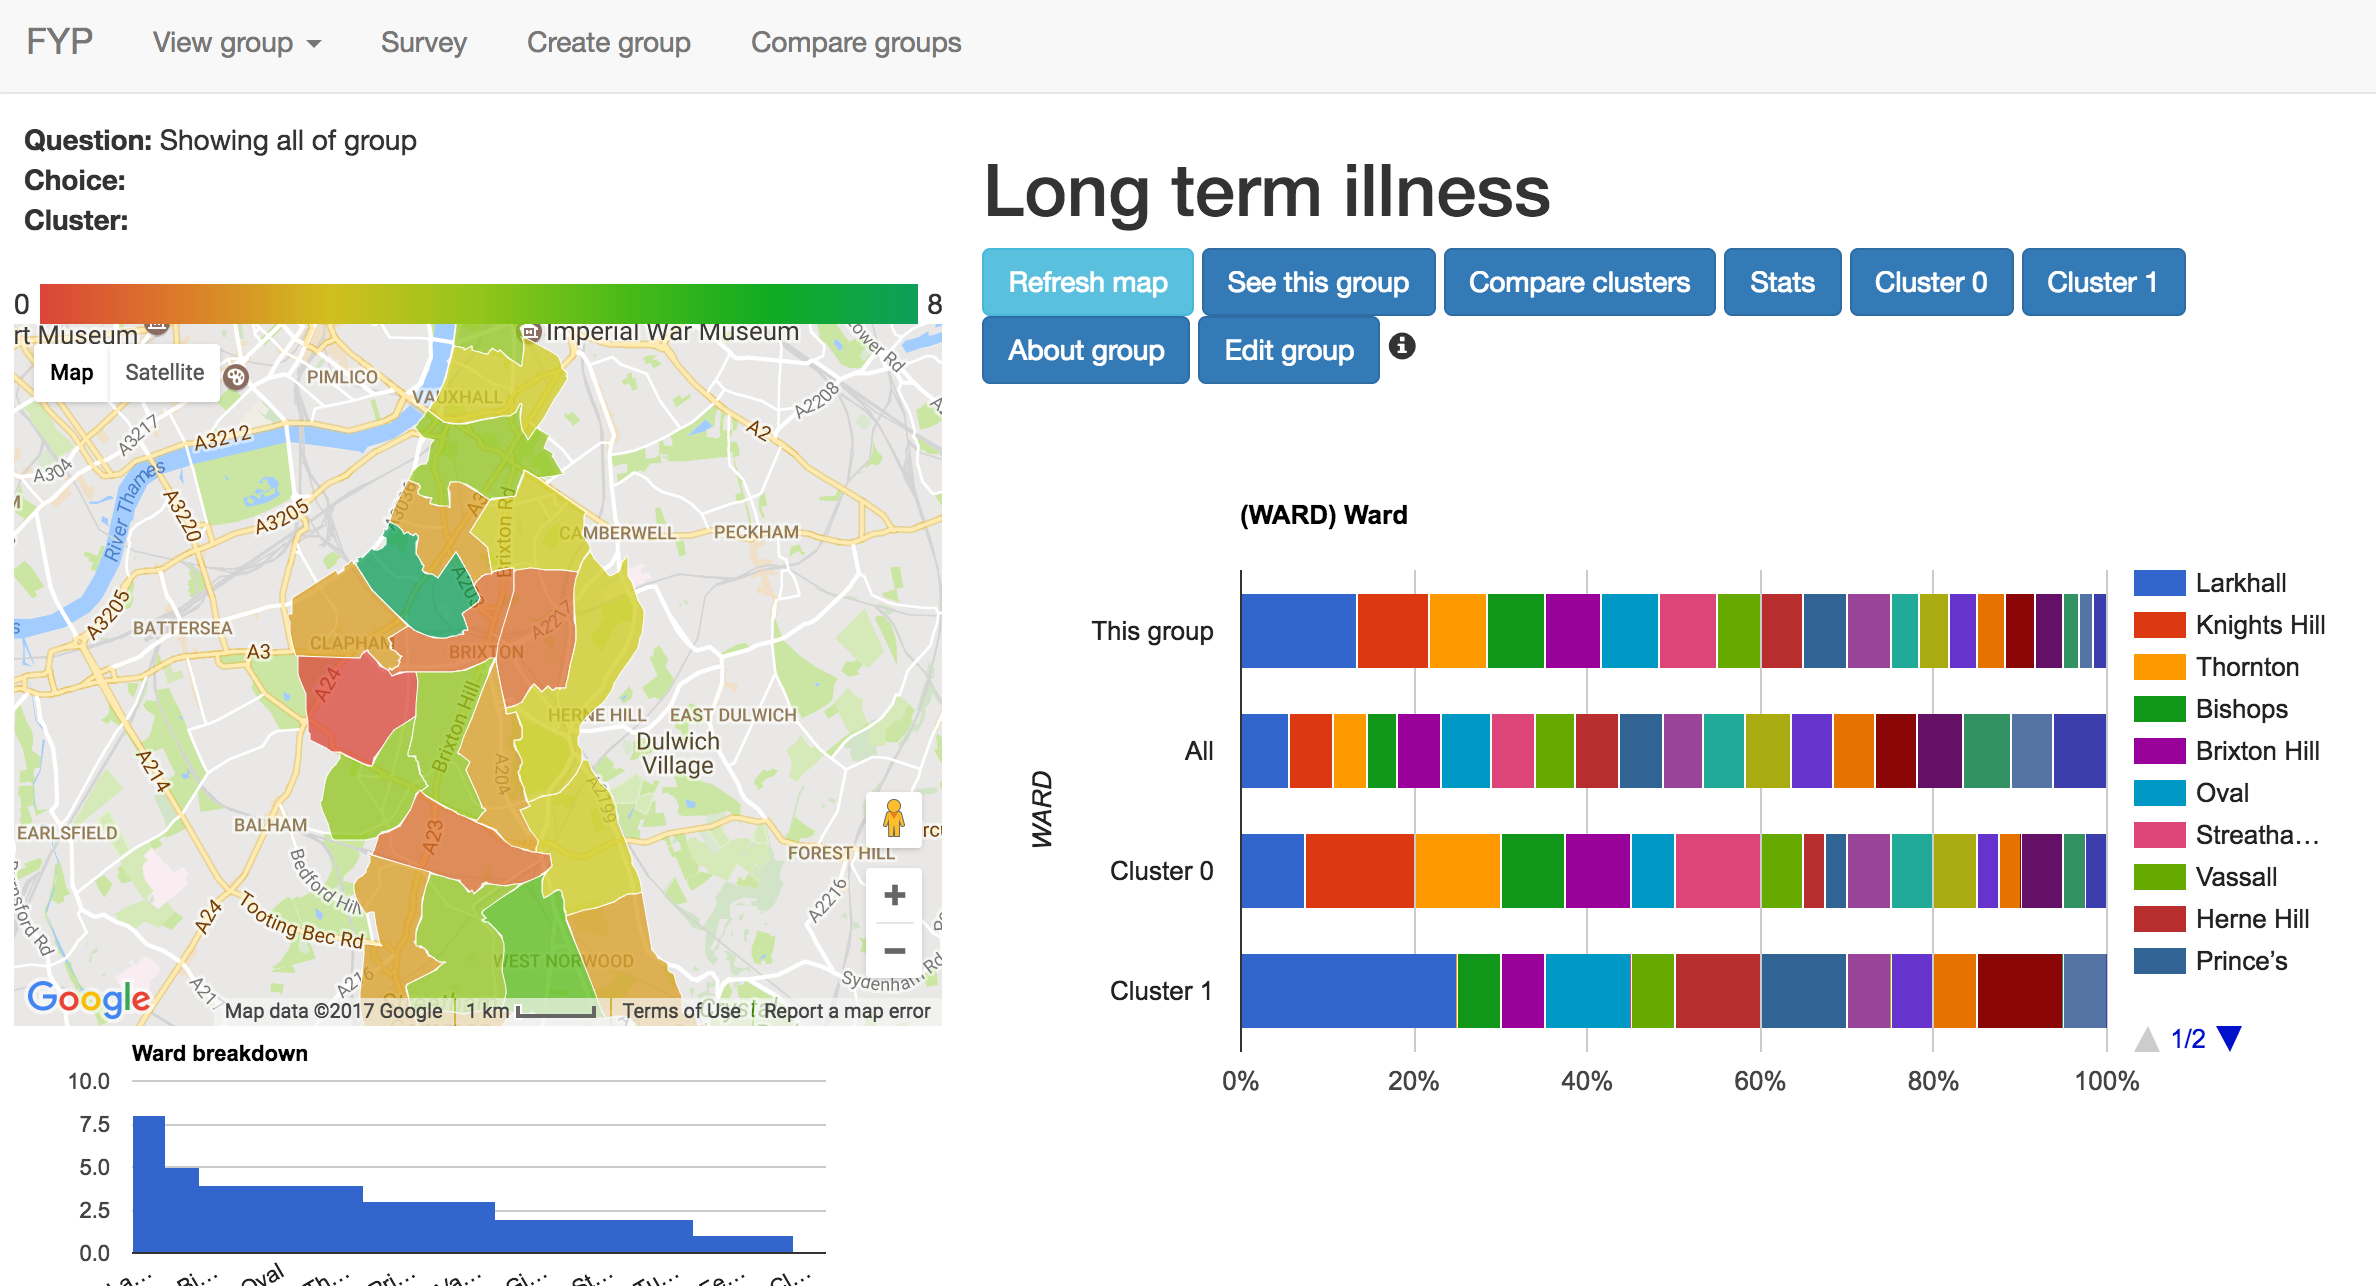
\includegraphics[scale=0.3]{comparisonpage}
\caption{Screenshot of the cluster\_compare page}
\label{fig:comparisonpage}
\end{figure}

All charts are stacked bar charts. The click to display on map feature is applicable to these charts as well.

\subsection{Comparison of groups}
On the right-hand side of the page (see figure \ref{fig:groupcompare}), the charts generated from the All group with the same method as in a group\_detail page. However, the left-hand side of the page is a bar chart of the group\textquotesingle s percent difference from the whole survey population. As with a group\textquotesingle s Detail page, clicking a piece of data on a chart will instigate a change in the left-hand side bar chart.\par

The percent difference is calculated using the equation found in the Design chapter (see section \ref{sec:interfacedesign})

\begin{figure}[h]
\centering
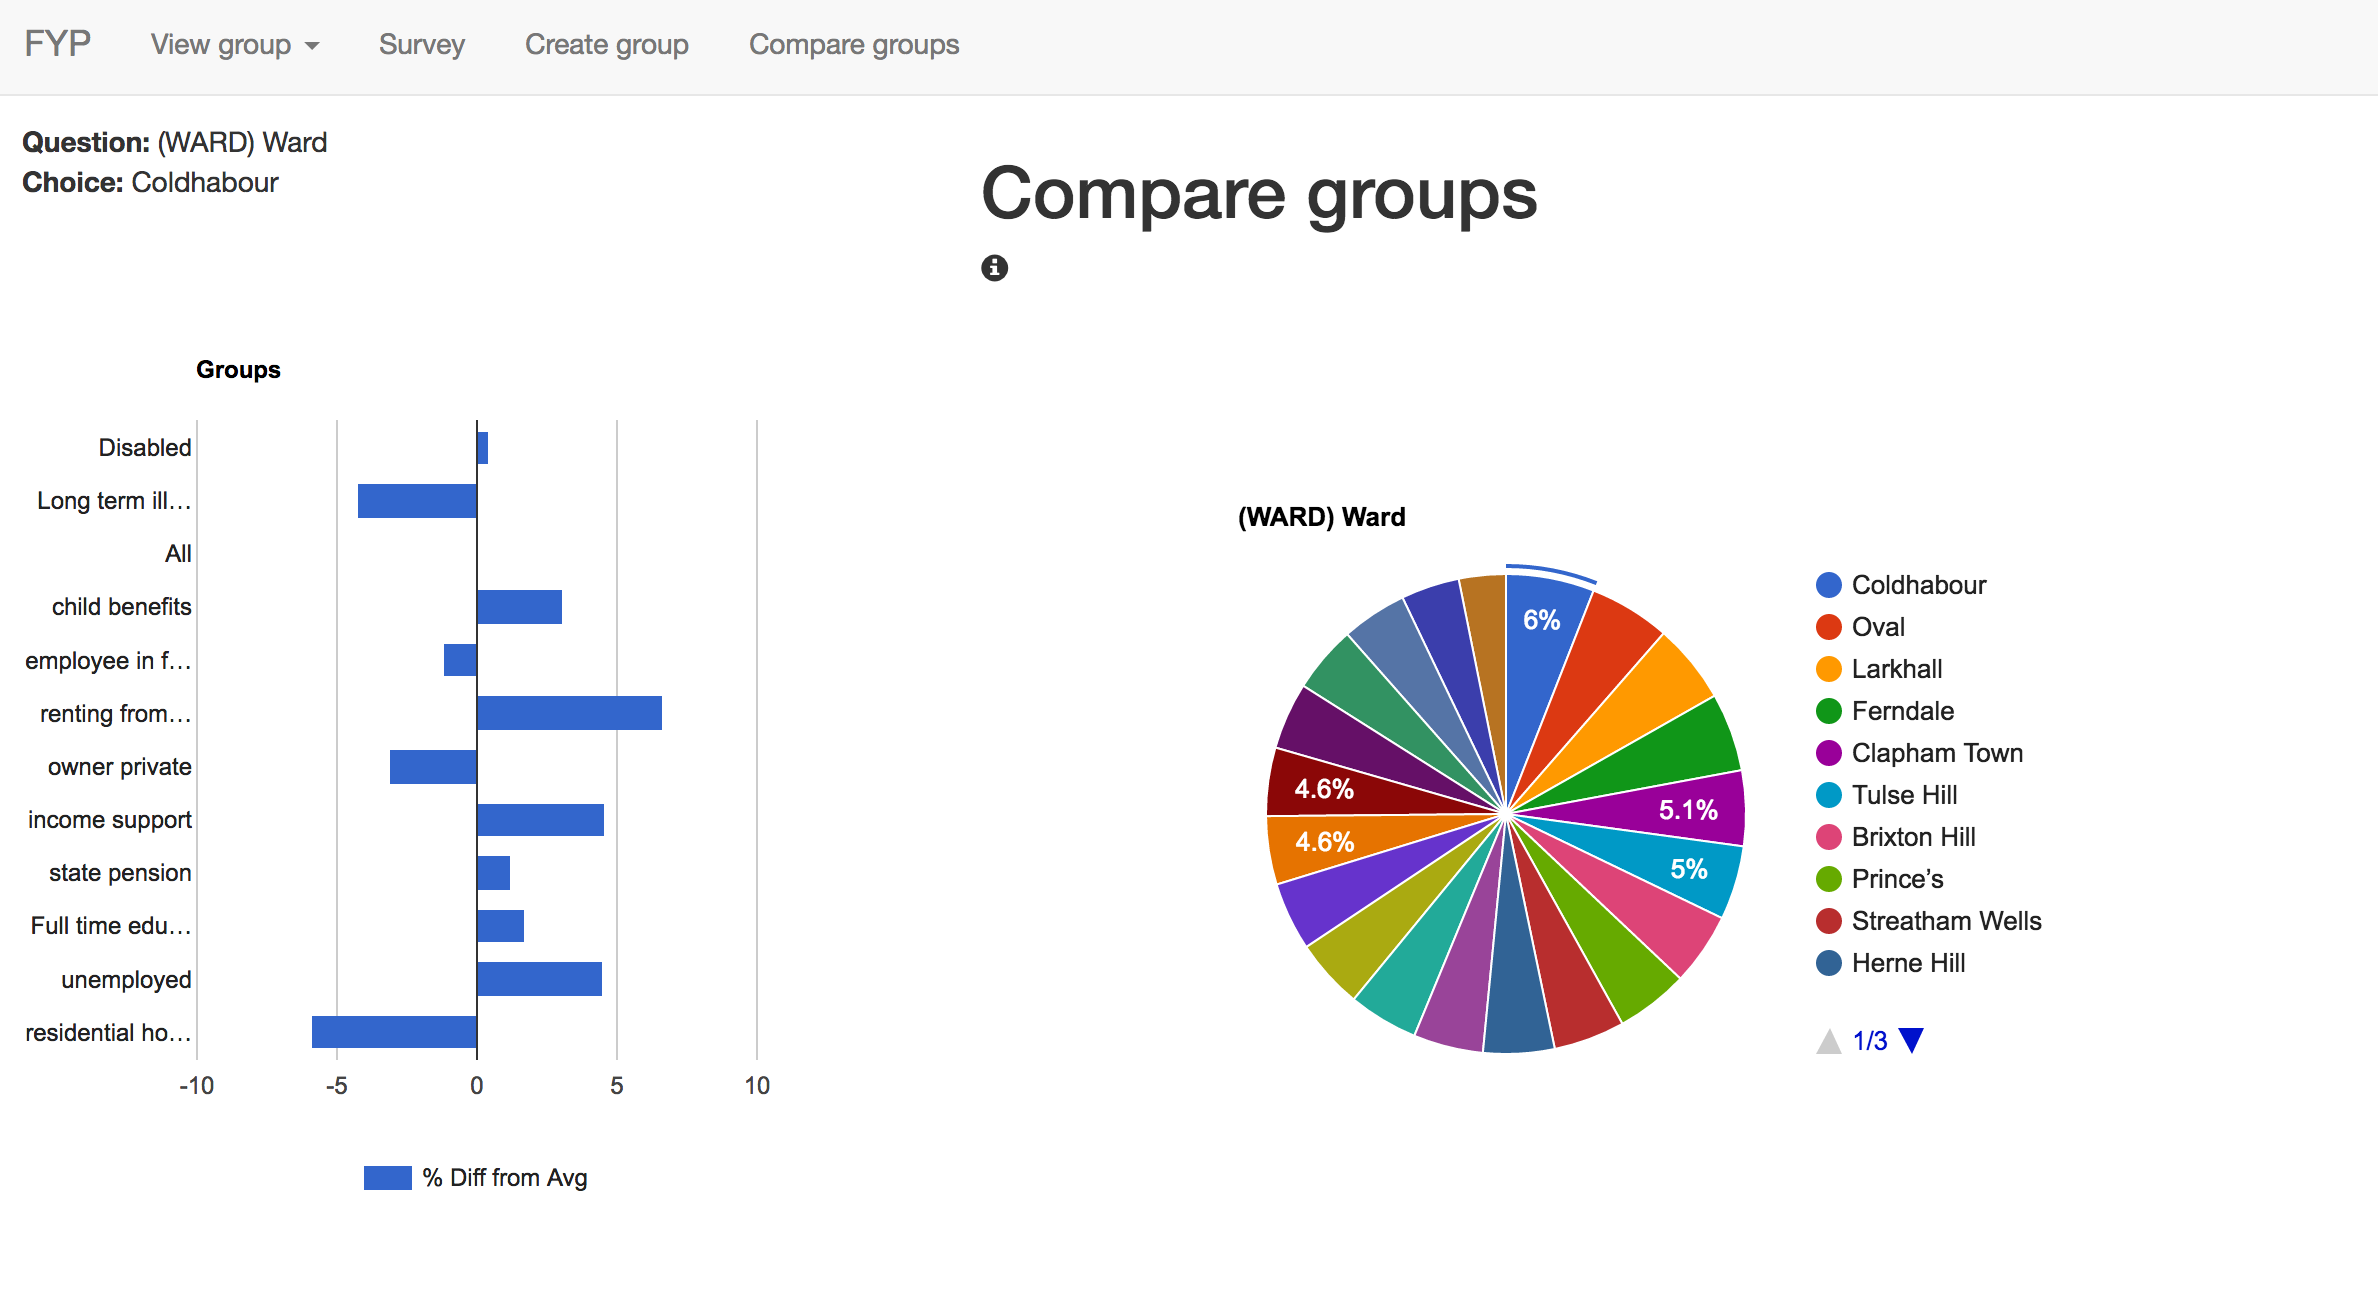
\includegraphics[scale=0.3]{groupcompare}
\caption{Screenshot of the group\_compare page}
\label{fig:groupcompare}
\end{figure}

\subsection{Clustering algorithm}

Each group was clustered according to the number of clusters set by the user in the Stats page. The default number of clusters is 1. K-modes clustering (citation) was used since it is more effective than k-means clustering to cluster categorical data, which the survey data is mainly composed of.\par

The results of clustering are stored in the database. The Subcluster Django model created the database table with fields: serial (i.e. serial of row in Survey data), group (i.e. Cluster model) and cluster (i.e. id of cluster). Should the number of clusters be changed by the user, the Subcluster records of the group will be deleted and replaced. If the clusters are queried, then the system will query the Subcluster database table so that the clusters remain the same.

\begin{figure}[h]
\centering
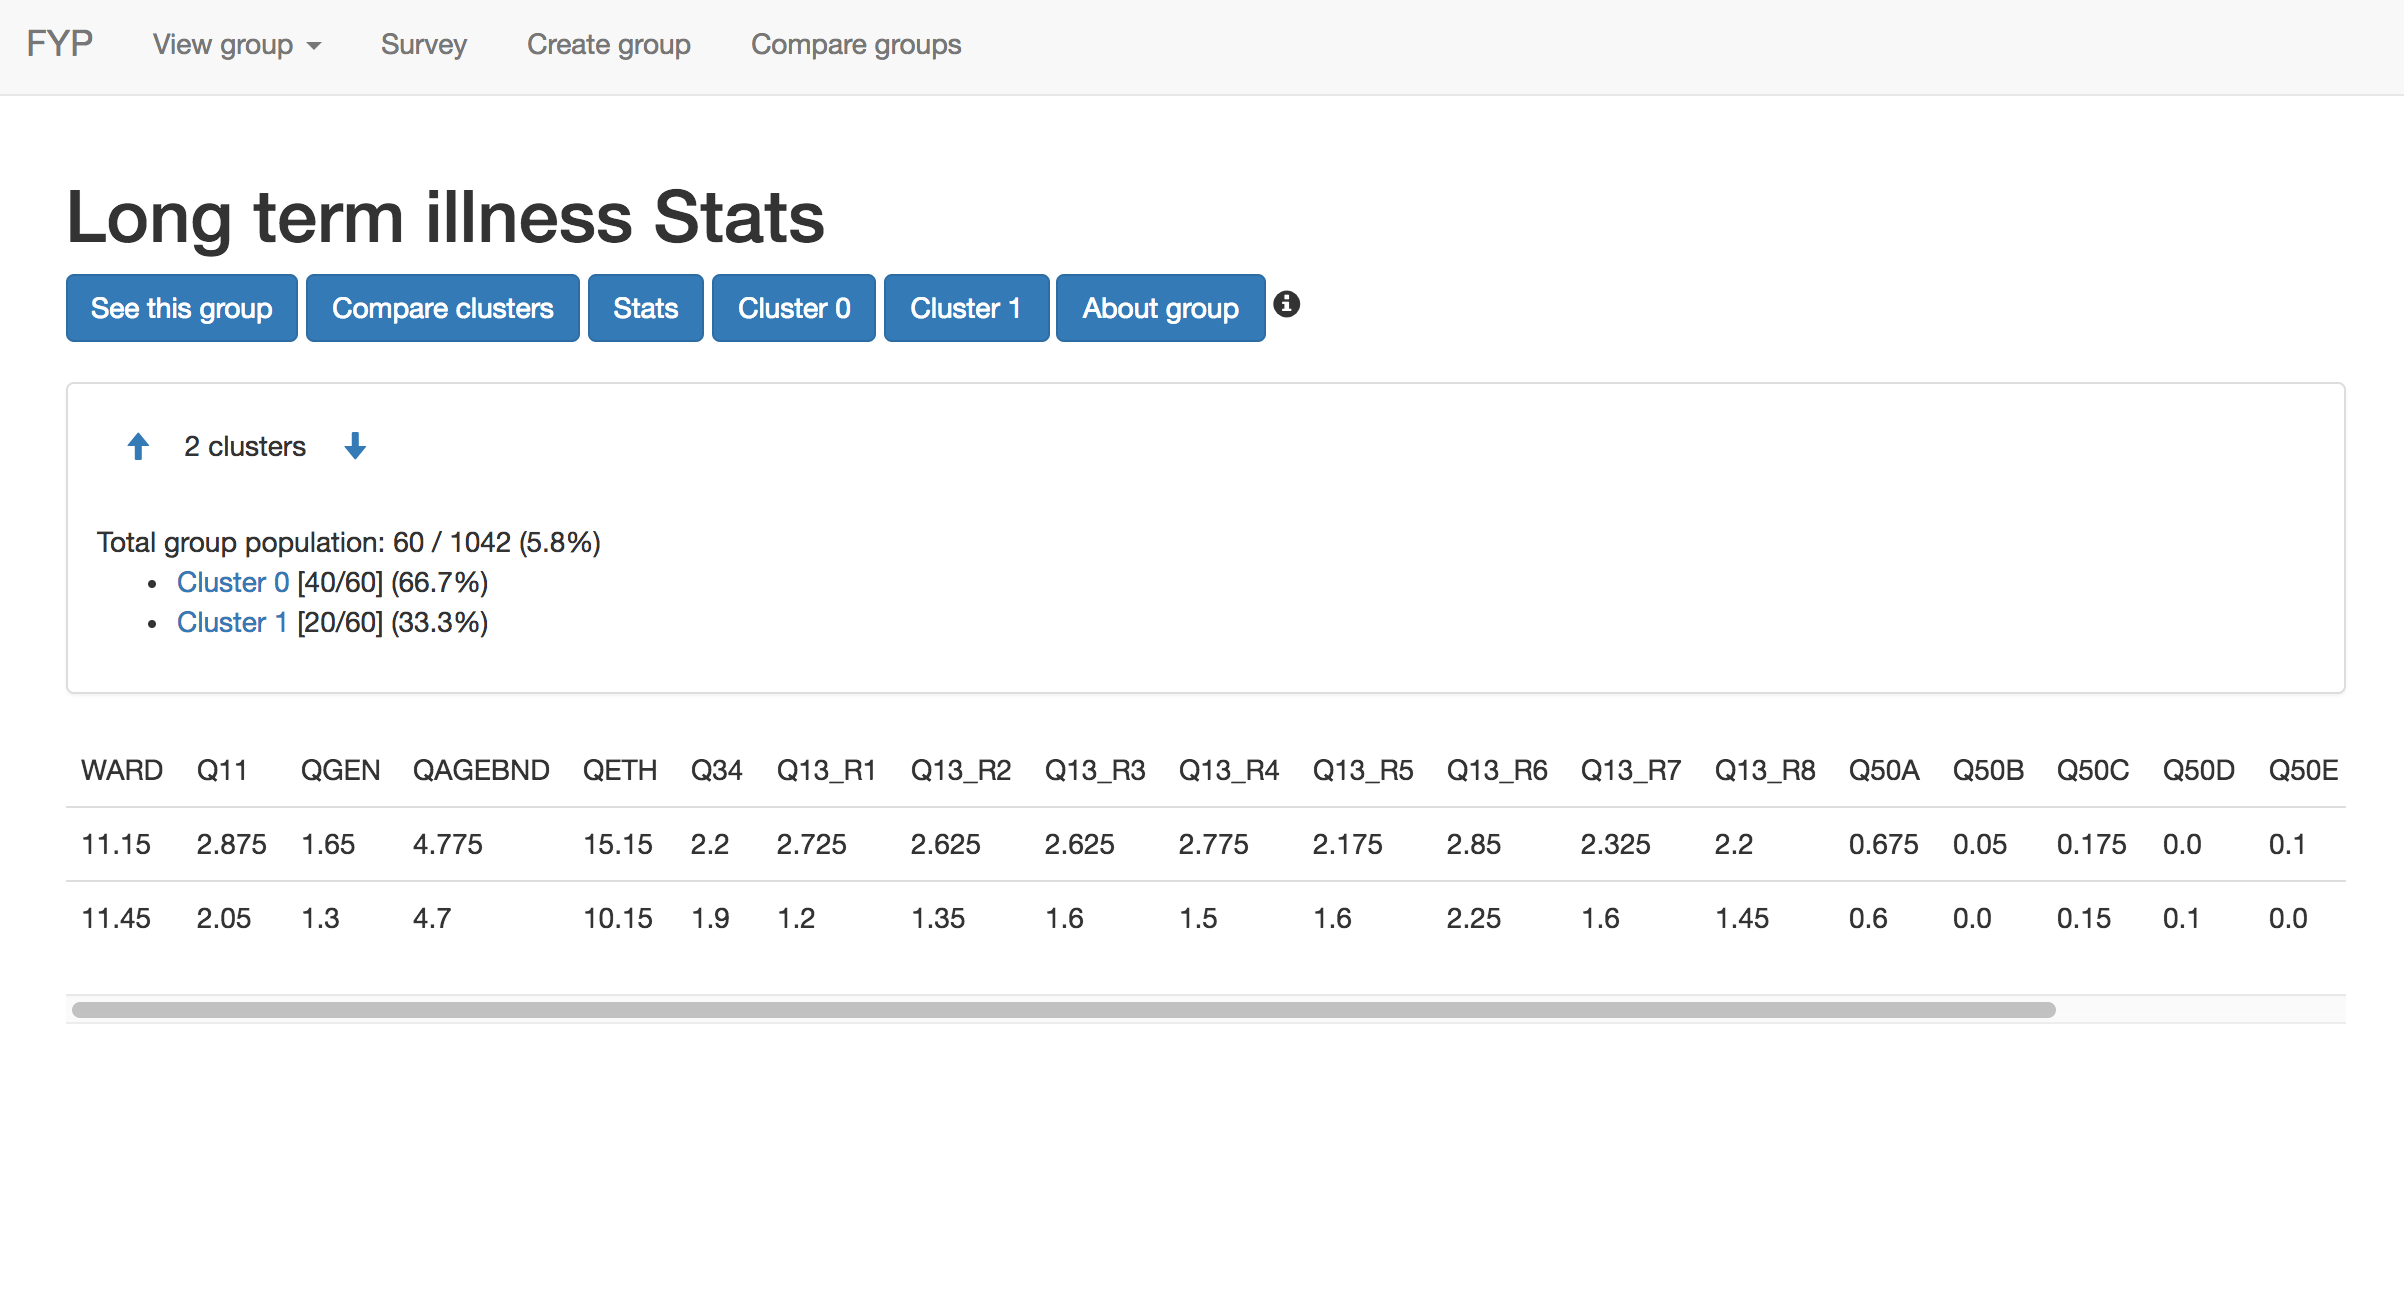
\includegraphics[scale=0.3]{clusterstats}
\caption{Screenshot of the cluster\_stats page}
\label{fig:clustestats}
\end{figure}


\subsection{Resource question page}
Similar to the clusters\_compare page and implemented with a similar Python operation, the survey question page displays more than one group in the same chart. 

\begin{figure}[h]
\centering
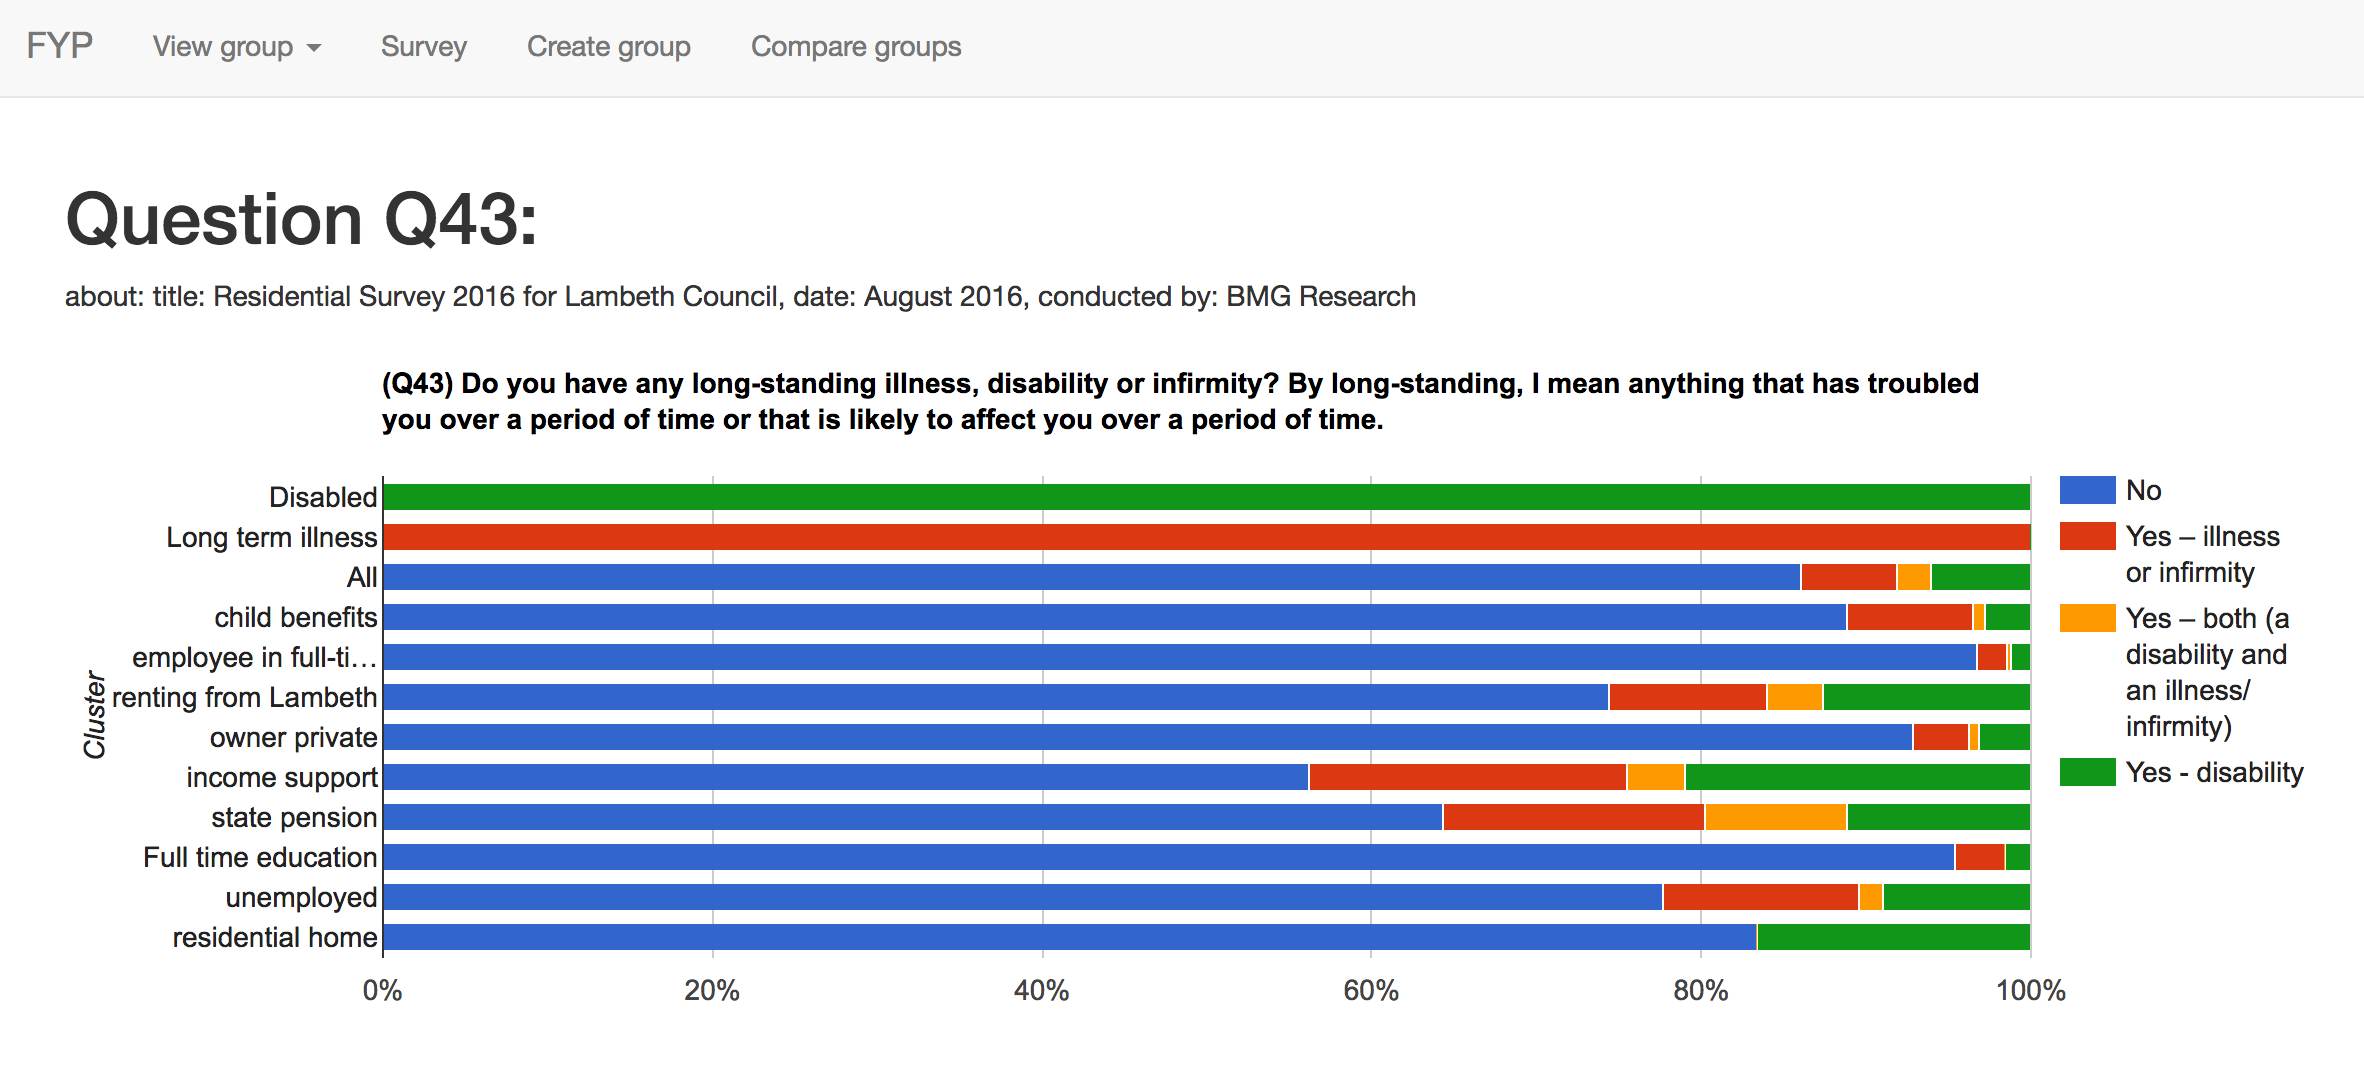
\includegraphics[scale=0.3]{surveyquestion}
\caption{Screenshot of the resource\_datafield page}
\label{fig:surveyquestion}
\end{figure}

\section{Testing}
To be continued